%%%%%%%%%%%%%%%%%%%%%%%%%%%%%%%%%%%%%%%%%
% Wenneker Article
% LaTeX Template
% Version 2.0 (28/2/17)
%
% This template was downloaded from:
% http://www.LaTeXTemplates.com
%
% Authors:
% Vel (vel@LaTeXTemplates.com)
% Frits Wenneker
%
% License:
% CC BY-NC-SA 3.0 (http://creativecommons.org/licenses/by-nc-sa/3.0/)
%
%%%%%%%%%%%%%%%%%%%%%%%%%%%%%%%%%%%%%%%%%

%----------------------------------------------------------------------------------------
%	PACKAGES AND OTHER DOCUMENT CONFIGURATIONS
%----------------------------------------------------------------------------------------

\documentclass[12pt, a4paper]{article} % 10pt font size (11 and 12 also possible), A4 paper (letterpaper for US letter) and two column layout (remove for one column)

%%%%%%%%%%%%%%%%%%%%%%%%%%%%%%%%%%%%%%%%%
% Wenneker Article
% Structure Specification File
% Version 1.0 (28/2/17)
%
% This file originates from:
% http://www.LaTeXTemplates.com
%
% Authors:
% Frits Wenneker
% Vel (vel@LaTeXTemplates.com)
%
% License:
% CC BY-NC-SA 3.0 (http://creativecommons.org/licenses/by-nc-sa/3.0/)
%
%%%%%%%%%%%%%%%%%%%%%%%%%%%%%%%%%%%%%%%%%

%----------------------------------------------------------------------------------------
%	PACKAGES AND OTHER DOCUMENT CONFIGURATIONS
%----------------------------------------------------------------------------------------

\usepackage[english]{babel} % English language hyphenation

\usepackage{microtype} % Better typography

\usepackage{amsmath,amsfonts,amsthm} % Math packages for equations

\usepackage[svgnames]{xcolor} % Enabling colors by their 'svgnames'

\usepackage[hang, small, labelfont=bf, up, textfont=it]{caption} % Custom captions under/above tables and figures

\usepackage{booktabs} % Horizontal rules in tables

\usepackage{lastpage} % Used to determine the number of pages in the document (for "Page X of Total")

\usepackage{graphicx} % Required for adding images

\usepackage{enumitem} % Required for customising lists
\setlist{noitemsep} % Remove spacing between bullet/numbered list elements

\usepackage{sectsty} % Enables custom section titles
\allsectionsfont{\usefont{OT1}{phv}{b}{n}} % Change the font of all section commands (Helvetica)

%----------------------------------------------------------------------------------------
%	MARGINS AND SPACING
%----------------------------------------------------------------------------------------

\usepackage{geometry} % Required for adjusting page dimensions

\geometry{
	top=1cm, % Top margin
	bottom=1.5cm, % Bottom margin
	left=2cm, % Left margin
	right=2cm, % Right margin
	includehead, % Include space for a header
	includefoot, % Include space for a footer
	%showframe, % Uncomment to show how the type block is set on the page
}

\setlength{\columnsep}{7mm} % Column separation width

%----------------------------------------------------------------------------------------
%	FONTS
%----------------------------------------------------------------------------------------

\usepackage[T1]{fontenc} % Output font encoding for international characters
\usepackage[utf8]{inputenc} % Required for inputting international characters

\usepackage{XCharter} % Use the XCharter font

%----------------------------------------------------------------------------------------
%	HEADERS AND FOOTERS
%----------------------------------------------------------------------------------------

\usepackage{fancyhdr} % Needed to define custom headers/footers
\pagestyle{fancy} % Enables the custom headers/footers

\renewcommand{\headrulewidth}{0.0pt} % No header rule
\renewcommand{\footrulewidth}{0.4pt} % Thin footer rule

\renewcommand{\sectionmark}[1]{\markboth{#1}{}} % Removes the section number from the header when \leftmark is used

%\nouppercase\leftmark % Add this to one of the lines below if you want a section title in the header/footer

% Headers
\lhead{} % Left header
\chead{\textit{\thetitle}} % Center header - currently printing the article title
\rhead{} % Right header

% Footers
\lfoot{} % Left footer
\cfoot{} % Center footer
\rfoot{\footnotesize Page \thepage\ of \pageref{LastPage}} % Right footer, "Page 1 of 2"

\fancypagestyle{firstpage}{ % Page style for the first page with the title
	\fancyhf{}
	\renewcommand{\footrulewidth}{0pt} % Suppress footer rule
}

%----------------------------------------------------------------------------------------
%	TITLE SECTION
%----------------------------------------------------------------------------------------

\newcommand{\authorstyle}[1]{{\large\usefont{OT1}{phv}{b}{n}\color{DarkRed}#1}} % Authors style (Helvetica)

\newcommand{\institution}[1]{{\footnotesize\usefont{OT1}{phv}{m}{sl}\color{Black}#1}} % Institutions style (Helvetica)

\usepackage{titling} % Allows custom title configuration

\newcommand{\HorRule}{\color{DarkGoldenrod}\rule{\linewidth}{1pt}} % Defines the gold horizontal rule around the title

\pretitle{
	\vspace{-30pt} % Move the entire title section up
	\HorRule\vspace{10pt} % Horizontal rule before the title
	\fontsize{32}{36}\usefont{OT1}{phv}{b}{n}\selectfont % Helvetica
	\color{DarkRed} % Text colour for the title and author(s)
}

\posttitle{\par\vskip 15pt} % Whitespace under the title

\preauthor{} % Anything that will appear before \author is printed

\postauthor{ % Anything that will appear after \author is printed
	\vspace{10pt} % Space before the rule
	\par\HorRule % Horizontal rule after the title
	\vspace{20pt} % Space after the title section
}

%----------------------------------------------------------------------------------------
%	ABSTRACT
%----------------------------------------------------------------------------------------

\usepackage{lettrine} % Package to accentuate the first letter of the text (lettrine)
\usepackage{fix-cm}	% Fixes the height of the lettrine

\newcommand{\initial}[1]{ % Defines the command and style for the lettrine
	\lettrine[lines=3,findent=4pt,nindent=0pt]{% Lettrine takes up 3 lines, the text to the right of it is indented 4pt and further indenting of lines 2+ is stopped
		\color{DarkGoldenrod}% Lettrine colour
		{#1}% The letter
	}{}%
}

\usepackage{xstring} % Required for string manipulation

\newcommand{\lettrineabstract}[1]{
	\StrLeft{#1}{1}[\firstletter] % Capture the first letter of the abstract for the lettrine
	\initial{\firstletter}\textbf{\StrGobbleLeft{#1}{1}} % Print the abstract with the first letter as a lettrine and the rest in bold
}

%----------------------------------------------------------------------------------------
%	BIBLIOGRAPHY
%----------------------------------------------------------------------------------------

\usepackage[backend=bibtex,style=authoryear,natbib=true]{biblatex} % Use the bibtex backend with the authoryear citation style (which resembles APA)

\addbibresource{example.bib} % The filename of the bibliography

\usepackage[autostyle=true]{csquotes} % Required to generate language-dependent quotes in the bibliography
 % Specifies the document structure and loads requires packages

%----------------------------------------------------------------------------------------
%	ARTICLE INFORMATION
%----------------------------------------------------------------------------------------

\title{Sistemas de Recomendación} % The article title

\author{
	\authorstyle{Uayeb Caballero Rodríguez} % Authors
	\newline\newline % Space before institutions
	\institution{Universidad Nacional Autónoma de Honduras, Ciudad Universitaria, Honduras}\ % Institution 1	
}

% Example of a one line author/institution relationship
%\author{\newauthor{John Marston} \newinstitution{Universidad Nacional Autónoma de México, Mexico City, Mexico}}

\date{\today} % Add a date here if you would like one to appear underneath the title block, use \today for the current date, leave empty for no date

%----------------------------------------------------------------------------------------
\usepackage{cite}
\usepackage{amsfonts}
\usepackage{graphicx}
\usepackage{listings}




\begin{document}

\tableofcontents

\addtocontents{toc}{\hspace{-7.5mm} \textbf{Capítulos}}
\addtocontents{toc}{\hfill \textbf{Página} \par}
\addtocontents{toc}{\vspace{-2mm} \hspace{-7.5mm} \hrule \par}

\maketitle % Print the title

\thispagestyle{firstpage} % Apply the page style for the first page (no headers and footers)

%----------------------------------------------------------------------------------------
%	ABSTRACT
%----------------------------------------------------------------------------------------

\lettrineabstract{
	A recommender system is an Information Retrieval technology that improves access and proactively 
	recommends relevant items to users by considering the users’ explicitly mentioned preferences and 
	objective behaviors. A recommender system is one of the major techniques that handle information overload 
	problem of Information Retrieval by suggesting users with appropriate and relevant items. Today, 
	several recommender systems have been developed for different domains however, these are not precise 
	enough to fulfil the information needs of users. Therefore, it is necessary to build high quality recommender 
	systems. In designing such recommenders, designers face several issues and challenges that need 
	proper attention. This paper investigates and reports the current trends, issues, challenges, and research 
	opportunities in developing high-quality recommender systems. If properly followed, these issues and challenges 
	will introduce new research avenues and the goal towards fine-tuned and high-quality 
	recommender systems can be achieved.
}

%----------------------------------------------------------------------------------------
%	ARTICLE CONTENTS
%----------------------------------------------------------------------------------------

\section{Introduccion}

Los sistemas de recomendaciones son herramientas que generan recomendaciones sobre un determinado objeto de estudio, 
a partir de las preferencias y opiniones dadas por los usuarios. El uso de estos sistemas se está poniendo cada vez más de
moda en Internet debido a que son muy útiles para evaluar y filtrar la gran cantidad de información disponible en la
Web con objeto de asistir a los usuarios en sus procesos de búsqueda y recuperación de información. 
En este trabajo realizaremos una revisión de las características y aspectos fundamentales relacionados con el diseño, 
implementación y estructura de los sistemas de recomendaciones analizando distintas propuestas que han ido apareciendo 
en la literatura al respecto.

\section{Collaborative Filtering}

El Filtrado colaborativo (FC) es una técnica utilizada por algunos sistemas recomendadores. En general,
el filtrado colaborativo es el proceso de filtrado de información o modelos, que usa técnicas que implican 
la colaboración entre múltiples agentes, fuentes de datos, etc. \cite{two} Las aplicaciones del filtrado colaborativo 
suelen incluir conjuntos de datos muy grandes. Los métodos de filtrado colaborativo se han aplicado a muchos 
tipos de datos, incluyendo la detección y control de datos (como en la exploración mineral, sensores 
ambientales en áreas grandes o sensores múltiples, datos financieros) tales como instituciones de 
servicios financieros que integran diversas fuentes financieras, o en formato de comercio electrónico y 
aplicaciones web 2.0 donde el foco está en los datos del usuario, etc. Esta discusión se centra en el 
filtrado colaborativo para datos de usuario, aunque algunos de los métodos y enfoques pueden 
aplicarse a otras aplicaciones.

$\newline$

En el enfoque más reciente, el filtrado colaborativo es un método para hacer predicciones automáticas (filtrado) 
sobre los intereses de un usuario mediante la recopilación de las preferencias o gustos de información de muchos 
usuarios (colaborador). El Filtrado colaborativo se basa, en que si una persona A tiene la misma opinión que una 
persona B sobre un tema, A es más probable que tenga la misma opinión que B en otro tema diferente que la 
opinión que tendría una persona elegida azar. Por ejemplo, un sistema de recomendación basado en el 
filtrado colaborativo para televisión podría hacer predicciones acerca de los programas que le gustarían a un 
usuario a partir de una lista parcial de los gustos de ese usuario (gustos o disgustos). Notese que estas 
predicciones son específicas para el usuario, pero utilizan la información obtenida de muchos usuarios. 
Esto difiere del enfoque más simple de otorgarle una puntuación promedio (poco específico) para cada elemento de interés, 
por ejemplo sobre la base de su número de votos.

\subsection{Índice Jaccard}

El índice de Jaccard ( IJ ) o coeficiente de Jaccard ( IJ ) mide el grado de similitud entre dos conjuntos, sea cual sea el tipo de elementos.
$\newline$
La formulación es la siguiente:
$\newline$
J(A,B) = |A ${\cap}$ B| / |A ${\cup}$ B|

$\newline$
Es decir, la cardinalidad de la intersección de ambos conjuntos dividida por la cardinalidad de su unión.
Siempre toma valores entre 0 y 1, correspondiente este último a la igualdad total entre ambos conjuntos.
En ecología se usa para medir la similitud, disimilitud o distancias que existen entre dos 
estaciones de muestreo, con una formulación equivalente \cite{one}
$\newline$
$\newline$
Ahora miremos como aplicar esta formula con R, En primer lugar declararemos un dataframe de peliculas con sus rankings 
$\newline$
\begin{lstlisting}[language=R]

a <- data.frame(user = "A", HP1 = 4, HP2 = NA, HP3 = NA, 
                TW=1, SW1 = 1, SW2= NA, SW2 = NA)
b <- data.frame(user = "B", HP1 = 5, HP2 = 5, HP3 = 4, 
                TW=NA, SW1 = NA, SW2= NA, SW2 = NA)
c <- data.frame(user = "C", HP1 = NA, HP2 = NA, HP3 = NA, 
                TW=2, SW1 = 4, SW2= 5, SW2 = NA)
d <- data.frame(user = "D", HP1 = NA, HP2 = 3, HP3 = NA, 
                TW=NA, SW1 = NA, SW2= NA, SW2 = 3)

movies.rating <- rbind(a,b,c,d)

\end{lstlisting}
$\newline$
Ahora la funcion que trabaja especificamente con un dataframe definido como el anterior:
$\newline$
\begin{lstlisting}[language=R]

Jaccard <- function(data.set, user1, user2){
  
  u1 <- subset(data.set, user == user1)
  u2 <- subset(data.set, user == user2)
  
  u1 <- u1[, !(names(u1) %in% c("user"))]
  u2 <- u2[, !(names(u2) %in% c("user"))]
  
  union_ <- 0
  intersect_ <- 0
  
  for(name_ in names(u1)){
    
    if( !is.na(u1[,name_]) & !is.na(u2[,name_])){
      intersect_ <- intersect_ + 1
    }
    
    if( !is.na(u1[,name_]) | !is.na(u2[,name_])){
      union_ <- union_ + 1
    }
    
  }
  
  intersect_/union_
  
}
\end{lstlisting}

$\newline$

Ahora cuando probamos la similitud de A con B y A con C obtendriamos los siguientes resultados: 

$\newline$

$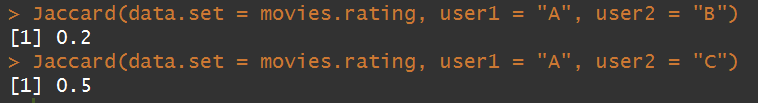
\includegraphics[width=3in]{jaccard.png}$

\subsection{Basado en memoria}

Este mecanismo utiliza los datos de las evaluaciones de los usuarios para calcular la similitud entre los usuarios o 
elementos. Esto se utiliza para hacer recomendaciones. Este fue de los primeros mecanismos y se usa en muchos 
sistemas comerciales. Es fácil de implementar y es eficaz. Ejemplos típicos de este mecanismo son los FC basados en el 
vecino más cercano y recomendaciones de los N-primeros basadas en elementos o usuarios.\cite{memory} Por ejemplo, 
en los enfoques basados en el usuario, el valor de la evaluación del usuario u con respecto al elemento 
i se calcula como una agregación de las evaluaciones de usuarios similares para el elemento:
$\newline$
${\displaystyle r_{u,i}=agrr_{u^{\prime }\in U}r_{u^{\prime },i}}$
$\newline$
Donde U denota el conjunto de los mejores N usuarios que son más similares al usuario u con respecto a i. Algunos ejemplos de la función de agregación incluye:
$\newline$
$\newline$
${\displaystyle r_{u,i}={\frac {1}{N}}\sum \limits _{u^{\prime }\in U}r_{u^{\prime },i}}$
$\newline$
${\displaystyle r_{u,i}=k\sum \limits _{u^{\prime }\in U}sim(u,u^{\prime })r_{u^{\prime },i}}$
$\newline$
${\displaystyle r_{u,i}={\bar {r_{u}}}+k\sum \limits _{u^{\prime }\in U}sim(u,u^{\prime })(r_{u^{\prime },i}-{\bar {r_{u^{\prime }}}})}$
$\newline$
$\newline$

Donde k es un factor de normalización se define como
 ${\displaystyle k=1/\sum _{u^{\prime }\in U}|sim(u,u^{\prime })|}$
y ${\displaystyle {\bar {r_{u}}}}$ es el promedio de las evaluaciones del usuario u para todos los elementos que ha evaluado.
$\newline$
$\newline$
El algoritmo basado en vecindad calcula la similitud entre dos usuarios o elementos, produce una predicción para el usuario 
tomando el promedio ponderado de todas las evaluaciones. Calcular la similitud entre los elementos o usuarios es una parte
 importante de este enfoque. Múltiples mecanismos tales como la correlación de Pearson y la similitud basada 
 en el coseno entre vectores sirven para esto. La similitud de correlación de Pearson de dos usuarios x, y se define como

${\displaystyle sim(x,y)={\frac {\sum \limits _{i\in I_{xy}}(r_{x,i}-{\bar {r_{x}}})(r_{y,i}-{\bar {r_{y}}})}{\sqrt {\sum \limits _{i\in I_{xy}}(r_{x,i}-{\bar {r_{x}}})^{2}\sum \limits _{i\in I_{xy}}(r_{y,i}-{\bar {r_{y}}})^{2}}}}}$

donde Ixy es el conjunto de elementos evaluados por ambos usuarios. El enfoque basado en coseno define la similitud entre dos usuarios x e y como:

${\displaystyle \operatorname {sim} (x,y)=\cos({\vec {x}},{\vec {y}})={\frac {{\vec {x}}\cdot {\vec {y}}}{||{\vec {x}}||\times ||{\vec {y}}||}}={\frac {\sum \limits _{i\in I_{xy}}r_{x,i}r_{y,i}}{{\sqrt {\sum \limits _{i\in I_{x}}r_{x,i}^{2}}}{\sqrt {\sum \limits _{i\in I_{y}}r_{y,i}^{2}}}}}}$

El algoritmo de recomendación basado en los N-primeros usuarios identifica los k más similares al usuarios actual usando 
el modelo de similitud basado en vectores. Después de que los k usuarios más similares se encuentran, 
sus correspondientes matrices de usuario- elementos se agregan para identificar el conjunto de elementos que se 
recomiendan. Un método popular para encontrar a los usuarios similares es el, que implementa el en tiempo lineal. 
Las ventajas de este enfoque incluyen: la interpretación de los resultados, lo cual es un aspecto importante 
de los sistemas de recomendación, es fácil de crear y utilizar; los nuevos datos se pueden agregar fácilmente y 
de forma incremental, no es necesario considerar el contenido de los elementos que se recomiendan, y mecanismo escala 
adecuadamente con elementos reevaluados. Hay varias desventajas con este enfoque. En primer lugar, depende de las
puntuaciones de las personas. En segundo lugar, su rendimiento disminuye cuando los datos son dispersos, lo cual 
es frecuente en elementos relacionados con la web. Esto evita la escalabilidad de este enfoque y tiene problemas 
con grandes conjuntos de datos. A pesar de que puede manejar eficientemente los nuevos usuarios porque cuenta 
con una estructura de datos, añadiendo nuevos elementos se hace más complicada, ya que la representación 
general se basa en un espacio vectorial específico. Para ello sería necesario incluir el nuevo elemento y 
volver a insertar todos los elementos de la estructura.
$\newline$
Para hacer experimentos en R con esto necesitamos de los siguientes paquetes
$\newline$
$\newline$

\begin{lstlisting}[language=R]

install.packages("recommenderlab")
install.packages("recosystem")

\end{lstlisting}

$\newline$
$\newline$
Para probar el codigo
$\newline$
$\newline$

\begin{lstlisting}[language=R]

library(recommenderlab)
library(recosystem)


#Building model
model <- Recommender(real_ratings, method = "IBCF", 
                     param=list(normalize = "center", 
					 method="Cosine", k=350))


#Making predictions 
prediction <- predict(model, real_ratings[1:5], type="ratings")
as(prediction, "matrix")[,1:8]

\end{lstlisting}
$\newline$
$\newline$
Y como resultado 
$\newline$
$\newline$

\begin{lstlisting}[language=R]
 m1       m2       m3       m4       m5       m6       m7      m8
u1       NA       NA 4.000000       NA       NA 4.400783       NA 3.73582
u2 4.264205 3.185612 3.172429 3.202051 3.581299 4.014510 3.253853 3.00000
u3 4.034784 3.794960 4.475967       NA 3.477293 4.171651 4.000000 5.00000
u4 4.319038       NA       NA       NA       NA 4.318060       NA      NA
u5 3.561104 1.783488 1.000000 2.638740 1.524747       NA 2.851991 3.00000
\end{lstlisting}
%------------------------------------------------


\section{Reducción de Dimensiones}

Para conjuntos de datos de alta dimensión (es decir, con número de dimensiones más de 10), reducción de la dimensión 
se realiza generalmente antes de la aplicación de un K-vecinos más cercanos (k-NN) con el fin de evitar los 
efectos de la maldición de la dimensionalidad. \cite{dimm}
$\newline$
Extracción de características y la reducción de la dimensión se puede combinar en un solo paso utilizando 
análisis de componentes principales (PCA), análisis discriminante lineal (LDA), o análisis de la correlación 
canónica (CCA) técnicas como un paso pre-procesamiento seguido por la agrupación de K-NN en vectores de 
características en el espacio reducido dimensión. En aprendizaje automático este proceso de pocas dimensiones 
también se llama incrustar.

$\newline$

Para conjuntos de datos muy altas dimensiones (por ejemplo, cuando se realiza la búsqueda de similitud de 
secuencias de vídeo en vivo, datos de ADN o de alta dimensión Series de tiempo) ejecutar un rápido 'aproximada' 
Búsqueda K-NN usando hash sensibles de localidad, "proyecciones aleatorias", "bocetos" u otras técnicas de búsqueda 
de similitud de alta dimensión de la VLDB caja de herramientas podría ser la única opción viable.

$\newline$$\newline$

Para Entrar a nuestra tecnica aplicada SVD es importante tenes claro los siguientes conceptos:

\subsection{Rango de una matriz}

El rango de una matriz es el número máximo de columnas (filas respectivamente) que son linealmente independientes. 
El rango fila y el rango columna siempre son iguales: este número es llamado simplemente rango de A 
(prueba más abajo). Comúnmente se expresa como rg(A).
$\newline$
El número de columnas independientes de una matriz A de m filas y n columnas es igual a la dimensión del 
espacio columna de A. También la dimensión del espacio fila determina el rango. El rango de A será, 
por tanto, un número no negativo, menor o igual que el mínimo entre m y n:

$\newline$

$\mathbb{A} \in M_{mxn} \to 0 \le rang(\mathbb{A}) \le min(m,n)$

%------------------------------------------------

\subsection{Eigen valores y  eigen espacios}

Formalmente, se definen los vectores propios y valores propios de la siguiente manera: Sea $A: V \to V$ n operador lineal en un cierto ${\displaystyle \scriptstyle} \scriptstyle {\mathbb  {K}}$-espacio vectorial V y v un vector no nulo en V. Si existe un escalar c tal que

$\newline$

${\displaystyle \mathbf {A} \mathbf {v} =c\mathbf {v} ,\qquad \mathbf {v} \neq \mathbf {0} ,c\in \mathbb {K} ,}$

$\newline$

entonces decimos que v es un vector propio del operador A, y su valor propio asociado es c. Observe que si v es un vector propio con el valor propio c 
entonces cualquier múltiplo diferente de cero de v es también un vector propio con el valor propio c. De hecho, todos los vectores propios 
con el valor propio asociado c junto con 0, forman un subespacio de V, el espacio propio para el valor propio c. 
Observe además que un espacio propio Z es un subespacio invariante de A, es decir dado w un vector en Z, el vector Aw también pertenece a Z.

%------------------------------------------------

\subsection{Proceso de ortogonalización de Gram-Schmidt}

El método de Gram-Schmidt se usa para hallar bases ortogonales (Espacio Euclideo no normalizado) de cualquier base no euclídea.
En primer lugar tenemos que:

${\displaystyle \mathbf {v} -{\langle \mathbf {v} ,\mathbf {u} \rangle  \over \langle \mathbf {u} ,\mathbf {u} \rangle }\mathbf {u} =\mathbf {v} -\mathrm {proy} _{\mathbf {u} }\,(\mathbf {v} )}$

Es un vector ortogonal a ${\displaystyle \mathbf {u} }$ . Entonces, dados los vectores ${\displaystyle \mathbf {v} _{1},\dots ,\mathbf {v} _{n}}$  , se define:

${\displaystyle \mathbf {u} _{1}=\mathbf {v} _{1},}$

${\displaystyle \mathbf {u} _{2}=\mathbf {v} _{2}-{\langle \mathbf {v} _{2},\mathbf {u} _{1}\rangle \over \langle \mathbf {u} _{1},\mathbf {u} _{1}\rangle }\mathbf {u} _{1},}$

${\displaystyle \mathbf {u} _{3}=\mathbf {v} _{3}-{\langle \mathbf {v} _{3},\mathbf {u} _{1}\rangle \over \langle \mathbf {u} _{1},\mathbf {u} _{1}\rangle }\mathbf {u} _{1}-{\langle \mathbf {v} _{3},\mathbf {u} _{2}\rangle \over \langle \mathbf {u} _{2},\mathbf {u} _{2}\rangle }\mathbf {u} _{2},}$

Generalizando en k:

${\displaystyle \mathbf {u} _{k}=\mathbf {v} _{k}-\sum _{j=1}^{k-1}{\langle \mathbf {v} _{k},\mathbf {u} _{j}\rangle \over \langle \mathbf {u} _{j},\mathbf {u} _{j}\rangle }\mathbf {u} _{j}} {\displaystyle \mathbf {u} _{k}=\mathbf {v} _{k}-\sum _{j=1}^{k-1}{\langle \mathbf {v} _{k},\mathbf {u} _{j}\rangle  \over \langle \mathbf {u} _{j},\mathbf {u} _{j}\rangle }\mathbf {u} _{j}}$

%------------------------------------------------

\subsection{Descomposición en valores singulares}

En álgebra lineal, la descomposición en valores singulares de una matriz real o compleja es una factorización de 
la misma con muchas aplicaciones en estadística y otras disciplinas.

Dada una matriz real ${\displaystyle A\in \Re ^{m\times n}}$, los autovalores de la matriz cuadrada, 
simétrica y semidefinida positiva ${\displaystyle A^{T}A\in \Re ^{n\times n}}$ son siempre reales y mayores o iguales a cero. 
Teniendo en cuenta el producto interno canónico vemos que:

$\newline$

${\displaystyle \left(A^{T}A\right)^{T}=A^{T}\left(A^{T}\right)^{T}=A^{T}A}$. O sea que es simétrica
$\newline$
${\displaystyle (Ax,Ax)=x^{T}A^{T}Ax=||Ax||^{2}\geq 0}$ es decir ${\displaystyle A^{T}A\,}$ es semidefinida positiva, 
es decir, todos sus autovalores son mayores o iguales a cero.
$\newline$

Si ${\displaystyle \lambda _{i}\,}$  es el i-ésimo autovalor asociado al i-ésimo autovector, 
entonces ${\displaystyle \lambda _{i}\in \Re }$. Esto es una propiedad de las matrices simétricas.


%------------------------------------------------

\subsection{SVD con R}

\begin{lstlisting}[language=R]

A = as.matrix(data.frame(c(4,7,-1,8), c(-5,-2,4,2), c(-1,3,-3,6)))
A

     c.4..7...1..8. c..5...2..4..2. c..1..3...3..6.
[1,]              4              -5              -1
[2,]              7              -2               3
[3,]             -1               4              -3
[4,]              8               2               6

\end{lstlisting}

Ahora para aplicar SVD podemos usar la funcion incluida en R

\begin{lstlisting}[language=R]
A.svd <- svd(A)
A.svd

d
[1] 13.161210  6.999892  3.432793

u
           [,1]       [,2]        [,3]
[1,] -0.2816569  0.7303849 -0.42412326
[2,] -0.5912537  0.1463017 -0.18371213
[3,]  0.2247823 -0.4040717 -0.88586638
[4,] -0.7214994 -0.5309048  0.04012567

v

           [,1]        [,2]       [,3]
[1,] -0.8557101  0.01464091 -0.5172483
[2,]  0.1555269 -0.94610374 -0.2840759
[3,] -0.4935297 -0.32353262  0.8073135

\end{lstlisting}


\subsection{SVD con R, paso a paso}

\begin{lstlisting}[language=R]
ATA <- t(A) %*% A
ATA

##                 c.4..7...1..8. c..5...2..4..2. c..1..3...3..6.
## c.4..7...1..8.             130             -22              68
## c..5...2..4..2.            -22              49              -1
## c..1..3...3..6.             68              -1              55

ATA.e <- eigen(ATA)
v.mat <- ATA.e$vectors
v.mat

##            [,1]        [,2]       [,3]
## [1,]  0.8557101 -0.01464091 -0.5172483
## [2,] -0.1555269  0.94610374 -0.2840759
## [3,]  0.4935297  0.32353262  0.8073135

v.mat[,1:2] <- v.mat[,1:2] * -1
v.mat

##            [,1]        [,2]       [,3]
## [1,] -0.8557101  0.01464091 -0.5172483
## [2,]  0.1555269 -0.94610374 -0.2840759
## [3,] -0.4935297 -0.32353262  0.8073135

AAT <- A %*% t(A)
AAT

##      [,1] [,2] [,3] [,4]
## [1,]   42   35  -21   16
## [2,]   35   62  -24   70
## [3,]  -21  -24   26  -18
## [4,]   16   70  -18  104

AAT.e <- eigen(AAT)
u.mat <- AAT.e$vectors
u.mat

##            [,1]       [,2]        [,3]       [,4]
## [1,] -0.2816569  0.7303849 -0.42412326 -0.4553316
## [2,] -0.5912537  0.1463017 -0.18371213  0.7715340
## [3,]  0.2247823 -0.4040717 -0.88586638  0.0379443
## [4,] -0.7214994 -0.5309048  0.04012567 -0.4426835

u.mat <- u.mat[,1:3]
r <- sqrt(ATA.e$values)
r <- r * diag(length(r))[,1:3]
r

##          [,1]     [,2]     [,3]
## [1,] 13.16121 0.000000 0.000000
## [2,]  0.00000 6.999892 0.000000
## [3,]  0.00000 0.000000 3.432793

svd.matrix <- u.mat %*% r %*% t(v.mat)
svd.matrix

##      [,1] [,2] [,3]
## [1,]    4   -5   -1
## [2,]    7   -2    3
## [3,]   -1    4   -3
## [4,]    8    2    6
\end{lstlisting}


\medskip
\newpage

\section{Conclusión}

La cantidad de algoritmos para construir sistemas de recomendacion son incontables, hoy en dia con el constante crecimiento de Internet
y con las distintas necesidades para retener los usuarios, los recommendation engines deben de ser mas precisos hasta el punto de 
dar la experiencia de personalizacion por usuario. tener este tipo de paradigmas hace que el costo computacional sea elevado en el 
caso de querer implementar tecnicas en base a filtros colaborativos, por lo que para datasets pequeños se recomienda su uso. lo bueno
de este tipo de tecnicas es que su interpretabilidad es mas rapida. para el caso de datasets muy grandes se recomiendan tecnicas que involucran 
reduccion de dimensiones como el caso de Descomposicion Espectral, SVD o ACP. Estos por su tecnica son mas rapidos de procesar
pero mas dificiles de interpretar. 

\newpage

%----------------------------------------------------------------------------------------
%	BIBLIOGRAPHY
%----------------------------------------------------------------------------------------

\begin{thebibliography}{9}


\printbibliography[title={Bibliography}] % Print the bibliography, section title in curly brackets
\bibitem{one}
Real, R., Vargas, J. M. (1996). The probabilistic basis of Jaccards index of similarity. Systematic biology, 45(3), 380-385

\bibitem{two}
Terveen, Loren; Hill, Will (2001). Beyond Recommender Systems: Helping People Help Each Other

\bibitem{memory}
Xiaoyuan Su, Taghi M. Khoshgoftaar, A survey of collaborative filtering techniques, Advances in Artificial Intelligence archive, 2009.

\bibitem{dimm}
Kevin Beyer, Jonathan Goldstein, Raghu Ramakrishnan, Uri Shaft (1999) "Cuando es" vecino más cercano "significativa? ". Base de datos Teoría-ICDT99 , 217-235

\end{thebibliography}

%----------------------------------------------------------------------------------------

\end{document}
